\section*{Abstract}

Users publish a high volume of information about real-world events on social
media almost instantly.
%
This makes social media a primary source for breaking news.
%
Some of these real-world events can end up having a very strong impact on the
network.  
%
The effect of such events can be analyzed from several perspectives, one of them
being the intensity and characteristics of the collective activity that it
produces in the social platform. 
%
We research 5,234 real-world news events encompassing 43 million messages
discussed on the Twitter microblogging service for approximately 1 year.  
%
We show empirically that exogenous news events naturally create collective
patterns of bursty behavior in combination with long periods of inactivity in
the network. 
%
This type of behavior agrees with other patterns previously observed in other
types of natural collective phenomena, as well as in individual human
communications. 
%
In addition, we propose a methodology to classify news events according to the
different levels of intensity in activity that they produce. 
%
In particular, we analyze the most highly active events and observe a consistent
and strikingly different collective reaction from users when they are exposed to
such events. 
%
This reaction is independent of an event's reach and scope.  
%
We further observe that extremely high-activity events have characteristics that
are quite distinguishable at the beginning stages of their outbreak.  
%
This allows us to predict with high precision, the top 8\% of events that will
have the most impact in the social network by just using the first 5\% of the
information of an event's lifetime evolution. 
%
This strongly implies that high-activity events are naturally prioritized
collectively by the social network, engaging users early on, way before they are
brought to the mainstream audience.


\section{Introduction}
% Motivation

Social media is now a primary source of breaking news information for millions
of users all over the
world~\cite{Kwak:2010,petrovic2013can,broersma2013twitter,tandoc2016most,Rogers:2013:DTT:2464464.2464511}.
%
Social media along with mobile internet devices have crowdsourced the
task of disseminating real-time information. 
%
As a result, both news media and news consumers have become inundated with much
more information than they can process. 
%
One possible way of handling this data overload is to find ways to filter and
prioritize information that has the potential of creating a strong collective
impact. 
%
Understanding and quickly identifying the type of reaction that certain
exogenous events will produce in social media, at both global and
local scales, can help in the understanding of collective human behavior.
%
This may as well as improve information delivery, journalistic coverage and
crisis management, among other things. 
%
We address this challenge by analyzing the properties of real-world news events
in social media, showing that they corroborate patterns previously identified in
other case studies of human communications. 
%
In addition, we present our main findings of how news events that produce
extremely high-activity can be clearly identified in the early stages of their
outbreak.

% Brief background on the problem
\subsection{Background}

The study of information propagation on the Web has sparked tremendous interest
in recent years. 
%
Current literature on the subject primarily considers the process through which
a {\em meme}, usually a piece of media (like a video, an image, or a specific
Web article), gains popularity
\cite{Castillo:2014,Szabo:2010,Lerman:2010,Tatar2014,Pinto:2013,Ahmed:2013,Li:2016:concept:drift,
Liu:2015:UN}. 
%
However, a meme represents a simple information unit and its propagation
behavior does not necessarily correspond to that of more complex information
such as news events. 
%
News events are usually diffused in the network in many different formats, e.g.,
a particular news story such as an {\em earthquake in Japan} can be communicated
through images, URLs, tweets, videos, etc. 
%
Therefore, current research can benefit from analyzing the effects of more
high-level forms of information. 

\begin{figure}
    \centering
    \begin{subfigure}[b]{\textwidth}
        \centering 
        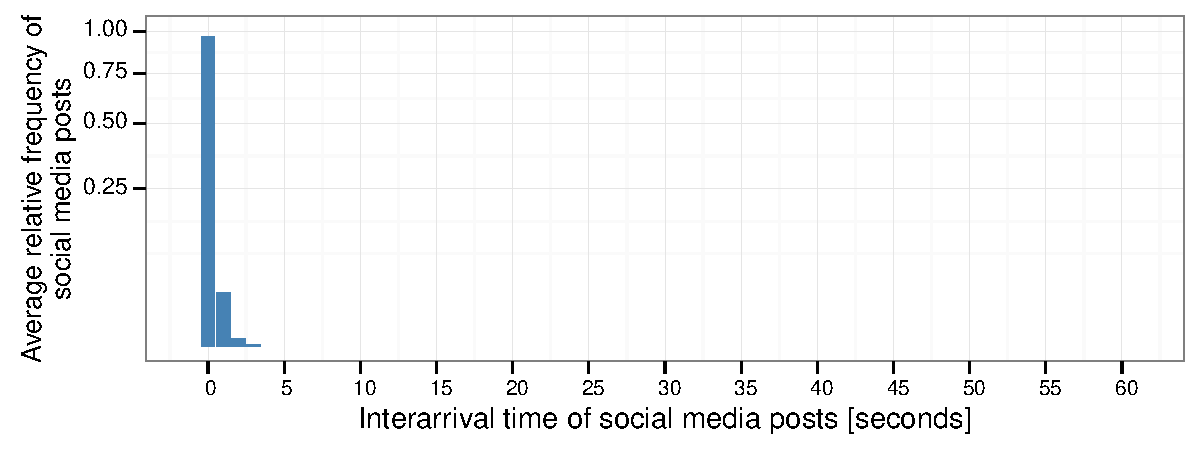
\includegraphics[width=.8\textwidth]{figures/high-activity/fig1a}
        \caption{Death of Nelson Mandela}
        \label{fig:hi:example-mandela}
    \end{subfigure}
    
    \begin{subfigure}[b]{\textwidth}
        \centering
        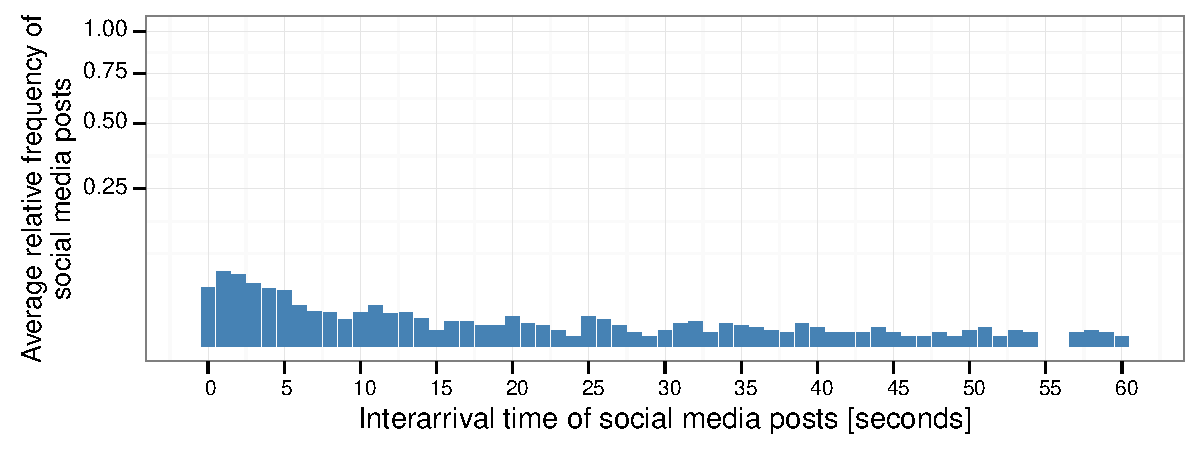
\includegraphics[width=.8\textwidth]{figures/high-activity/fig1b}
        \caption{One week after 2014 The Oscars}
        \label{fig:hi:example-oscars}
    \end{subfigure}

    \caption[Example histograms of time differences between tweets]{Histograms
        of the time differences between consecutive tweets in two example
        events: the death of Nelson Mandela (collected on 2013-12-05) and the
        commentary about the 2014 Oscars, several weeks after the main event
        (collected on 2014-03-23). Since there is a high concentration in the
        first histogram bin for the first histogram, we conclude that the social
        media posts for this event occur in cascades of quick successions,
        almost instantaneously. The arrival times of the posts on the second
        event are much more spread out. The $y$-axis is in square root scale.}
    \label{fig:hi:examples}
\end{figure}

Traditionally, the impact of information in on-line social networks has been
measured in relation to the total amount of attention that this subject receives
\cite{berger2012makes,iribarren2011branching,guerini2011exploring,mills2012virality,gaugaz2012predicting}.
%
That is, if a content posted in the network receives votes/comments/shares above
a certain threshold it is usually deemed as {\em viral} or {\em popular}.
%
Nevertheless, this notion of popularity or impact will favor only information
that produces very large volumes of social media messages. 
%
Naturally, global breaking news that has world-wide coverage and that produces a
high volume of activity in a short time should be considered as having a strong
impact on the network (Figure~\ref{fig:hi:example-mandela}).  
%
However, there are other types of events that can produce a similar reaction in
smaller on-line communities such as, for example, on users from a particular
country (e.g., the withdrawal of the main right wing presidential candidate in
Chile due to psychiatric problems, just before
elections~\cite{chile_elections}). 
%
Clearly, events of local scope do not produce as much social media activity as
events of global scope, but they can create a strong and immediate reaction from
users in local networks~\cite{ReisBOPKA15}. 
%
Conversely, there are large events which do not produce an intense reaction,
such as {\em The Oscars} (Figure~\ref{fig:hi:example-oscars}), which span a long
period of time and are discussed by social network users for weeks or even
months, but do not spark intense user activity. 
%
Therefore, it is reasonable to consider additional dimensions, than just volume,
when analyzing the impact of information in on-line communities.  

Prior research has shown that certain types of individual activities, such as
communications (studied in email exchanges), work patterns and entertainment,
follow a behavior of bursts of rapidly occurring actions followed by long
periods of inactivity~\cite{barabasi2005origin}, referred to as {temporally
inhomogeneous} behavior~\cite{karsai2012universal}.  
%
This type of behavior initially observed in individual activities, has also been
observed in relation to other naturally occurring types of collective phenomena
in human dynamics similar to processes seen in self-organized
criticality~\cite{karsai2012universal}.  
%
In particular, extremely high-activity bursty behavior seems to also occur in
critical situations, observed from the information flow in cell phone networks
during emergencies\cite{gao2014quantifying}.  
%
Although, there is research towards modeling this type of collective behavior
\cite{yan2013information} in on-line social networks, to the best of our
knowledge, it has not yet been analyzed quantitatively.





% when
% consulting journalists on how news media sources measure the impact of
% news, we learn that they too face the issue of not having a clear way
% to approach this problem.

% Our contributions

%\newtext{

\subsection{Contributions}

Our work focuses on high-activity events in social media produced by real-world
news, with the following contributions:
\begin{enumerate}

\item We introduce a methodology for modeling and classifying events in social
media, based on the intensity of the activity that they produce. 
%
This methodology is independent of the size and scope of the event, and is an
indicator of the impact that the event information had on the social network.

\item We show empirically that real-world news events produce collective
patterns of bursty behavior in the social network, in combination with long periods of
inactivity. 
%
Furthermore, we identify events for which most of their activity is concentrated
into very high-activity periods, we call these events {\em high-activity
events}.

\item We determine the existence of unique characteristics that differentiate
how high-activity events propagate in the social network.

\item We show that an important portion of high-activity events can be predicted
very early in their lifecycle, indicating that this type of information is
spontaneously identified and filtered collectively, early on, by social network
users.

\end{enumerate}
%}

%We focus on high-impact news events in social media, contributing by (i)
%\textcolor{blue}{defining a new concise way for measuring information impact that
%is independent of the size (whether large or small) and scope (whether
%local or global) of the event, but is representative of the urgency
%and immediacy of the reaction of users on the social media} (ii)
%determining the existence of unique characteristics that differentiate
%how high-impact exogenous events are propagated in the network, and
%(iii) show, through the creation of an early prediction model for
%high-impact events, that these types of news events are naturally
%identified and filtered by the network at very early stages of their
%outbreak.